\chapter{Realisierung des Prototypen}
Um eine bessere Aussage �ber die Zukunftstauglichkeit von Distributed Ledger Technologien zu gewinnen, wird gemeinsam mit der IOTA Technologie ein Anwendungsfall prototypisch implementiert. Bei diesem Anwendungsfall handelt es sich um eine Tankstelle an der ein Auto m�glichst autonom den Tankvorgang startet und im Anschluss den anfallenden Betrag mit der Kryptow�hrung IOTA begleicht. Die kommende Ausf�hrung befasst sich mit der Implementation eines Prototypen.

Aus dem analytischen Teil folgt, dass zwischen Bitcoin und IOTA deutliche Unterschiede herrschen. F�r die Auswahl einer Distributed Ledger Technologie wurden Faktoren wie Best�tigungszeit und Transaktionsgeb�hren miteinbezogen. Ein weiterer Grund f�r die Auswahl einer Technologie war die Dokumentation ihrer Bibliotheken.

Aufgrund einer vorhandenen Dokumentation, schnellen Verifizierungen von Transaktionen und das fehlen einer Geb�hr wurde IOTA f�r die Implementierung ausgew�hlt.

\chapter{Fahrzeug - Client}
Das Programm soll f�r einen realit�tsnahen Anwendungsfall auf einem relativ leistungsschwachen System arbeiten k�nnen. Daher liegt es nahe f�r die Programmierung des Programmierteils, der f�r das Tanken und Bezahlen mit IOTAs zust�ndig ist, einen Raspberry Pi anzusteuern.

Der Raspberry Pi soll in dieser prototypischen Umsetzung die Steuereinheit eines zuk�nftigen Autos ersetzen. Es soll mittels zwei Kn�pfen bedienbar sein, die die Steuerelemente in der Armatur des Autos darstellen sollen.

Da der Anspruch an starke Rechenleistung in einem Auto nicht zu hoch sein sollte (um zum Beispiel Kosten zu minimieren) ist es sinnvoll, keinen IOTA Full-Node zu betrieben, sondern nur einen Light-Node, der die Arbeit an einen Full-Node delegiert. Die Limitation der Hardware-Ressourcen ist ein Grund f�r die Umsetzung auf einem Raspberry Pi.

Die Anforderungen an das Smartauto sind wie folgt:
\begin{itemize}
	\item Der Nutzer muss vor dem dem Tankvorgang �ber die Tankstelle informiert werden
	\item Der Nutzer soll mit einem Knopfdruck tanken k�nnen
	\item Der Nutzer soll mit einem Knopfdruck bezahlen k�nnen, ohne das weitere Eingaben notwendig sind
	\item Die Transaktion muss schnell von der Tankstelle validiert werden
\end{itemize}
An diese Anforderungen orientiert sich die folgende Umsetzung.


\section{Aufbau}
Unter diesem Aspekt wird der Aufbau und die Einrichtung der einzelnen Komponenten beschrieben die f�r die Umsetzung n�tig sind.

\subsection{Vorbedingungen}
Unter diesem Aspekt werden die Voraussetzungen f�r die Umsetzung der clientseitigen Tankanwendung beschrieben. Diese Vorbedingungen wurden genutzt um den Raspberry Pi so einzurichten und zu konfigurieren, damit das Ger�t die Anforderungen an das Programm erf�llen kann.

Um die prototypische Anwendung umsetzen zu k�nnen, werden folgende Komponenten genutzt:

\subsubsection{Raspberry Pi 3 Model B}
Auf dem Raspberry Pi wird die Anwendung ausgef�hrt, Daten des Benutzers verarbeitet und Anfragen auf Webservices vollzogen. Auch die Transaktionen von IOTAs sollen mithilfe des CPUs erstellt werden.

\subsubsection{Steckbrett}
Das Steckbrett dient der Verbindung von Bedienelementen mit den GPIO-Pins des Raspberry Pis. Die Kn�pfe f�r die Bedienung der Tank-Anwendung werden auf diesem befestigt und mit den GPIO-Pins elektronisch verbunden.

\subsubsection{Micro SD Karte}
Diese Speicherkarte wird f�r den Raspberry Pi gebraucht. Auf dieser befindet sich das Betriebssystem mit dem der Raspberry Pi erst genutzt werden kann. Auch das Programm und sonstige Benutzerdaten werden auf dieser Speicherkarte gespeichert.

\subsubsection{Micro USB Netzteil 5,1 Volt 3,1 Ampere}
Der Raspberry Pi muss mittels eines Micro USB Eingangs mit Strom versorgt werden. Das Netzteil sollte eine Ausgangsspannung von mindestens 5,1 Volt aufweisen und es werden mindestens 2,5 Ampere empfohlen\footnote{Nach https://www.raspberrypi.org/documentation/hardware/raspberrypi/power/README.md}.

\subsubsection{5x Weiblich-M�nnlich Kabel, 2x M�nnlich-M�nnlich Kabel}
Verbindungskabel f�r das Steckbrett um elektronische Komponenten miteinander zu Verbinden.

\subsubsection{2x Taster, 1x Rote LED}
Elektronische Komponenten um dem Benutzer der Anwendung Bedienelemente zur Verf�gung zu stellen. Die LED dient f�r ein visuelles Feedback.

\subsubsection{Widerst�nde 1x 330 Ohm, 2x 10.000 Ohm, 2x 1.000 Ohm}
Die Widerst�nde sind f�r den kontrollierten Stromfluss unentbehrlich und sie verhindern, dass die Komponenten durch zu hohen Stromfluss besch�digt werden.

\subsection{Einrichtung}
Um den Raspberry Pi so einzurichten, dass es m�glich ist, Anwendungen zu programmieren und zu testen, sollte dieser mittels eines HDMI-Kabels an einen Monitor angeschlossen werden. Weiterhin sollten Peripherieger�te wie Tastatur und Maus �ber die USB-Ausg�nge angeschlossen werden um sich durch die Bedienoberfl�che navigieren zu k�nnen. Doch damit das Ger�t vollst�ndig bedienbar wird, muss es mit einem Betriebssystem ausgestattet sein. Aufgrund von offiziellem Support seitens der Raspberry Pi Foundation [26](Quelle) wurde das Raspbian Betriebssystem f�r die Umsetzung ausgew�hlt. Bei Raspbian handelt es sich um ein, auf Linux basierendes Betriebssystem, welches von der Raspberry Pi Foundation ver�ffentlicht wurde.

Das Raspbian Betriebssystem muss auf die Micro SD Karte geladen werden, damit es f�r den Raspberry Pi zur Verf�gung steht. In folgenden Schritten wurde die Speicherkarte mit Raspbian beschrieben:
\begin{enumerate}
	\item Download von Raspbian (https://www.raspberrypi.org/downloads/)
	\item Gegebenenfalls .zip/.rar entpacken
	\item Speicherkarte in ein Kartenleseger�t stecken
	\item Mithilfe eines Brennprogramms die Imagedatei auf die Speicherkarte brennen (flashen)
\end{enumerate}

Die Speicherkarte ist nun formatiert und mit Raspbian ausgestattet, sie kann nun aus dem Kartenleseger�t genommen werden und in den Raspberry Pi gesteckt werden.

Nachdem das Ger�t zum ersten Mal gestartet wird, muss das Betriebssystem einmalig eingerichtet werden. Wenn dies geschehen ist, sollte man jegliche Software-Pakete in Raspbian updaten um m�gliche Fehler vorzubeugen. Dies kann mit folgenden Befehlen in dem Terminal des Betriebssystems vollzogen werden:

\begin{lstlisting}[language=bash]
> sudo apt-get update
> sudo apt-get dist-upgrade
\end{lstlisting}

\subsubsection{Steckbrett und GPIO-Pins}
Die Taster und LEDs m�ssen elektrisch mit den GPIO-Pins verbunden werden, um von dem Raspberry Pi angesprochen werden zu k�nnen. Die Taster stellen Kn�pfe auf der Armatur des Autos dar. Die LED dient daf�r, ein visuelles Feedback zu geben, zum Beispiel im Bezug auf die Tank-Anwendung ob nun getankt werden kann.

Daf�r ist es n�tzlich, mit dem Pin-Layout des Raspberry Pis vertraut zu sein. Mit dem Terminal-Befehl

\begin{lstlisting}[language=bash]
> pinout
\end{lstlisting}

ist es m�glich einen �berblick �ber das Layout des Raspberry Pis zu erhalten. Auch die Benennung der einzelnen Pins ist aufgef�hrt.

\begin{figure}[H]%
\centering
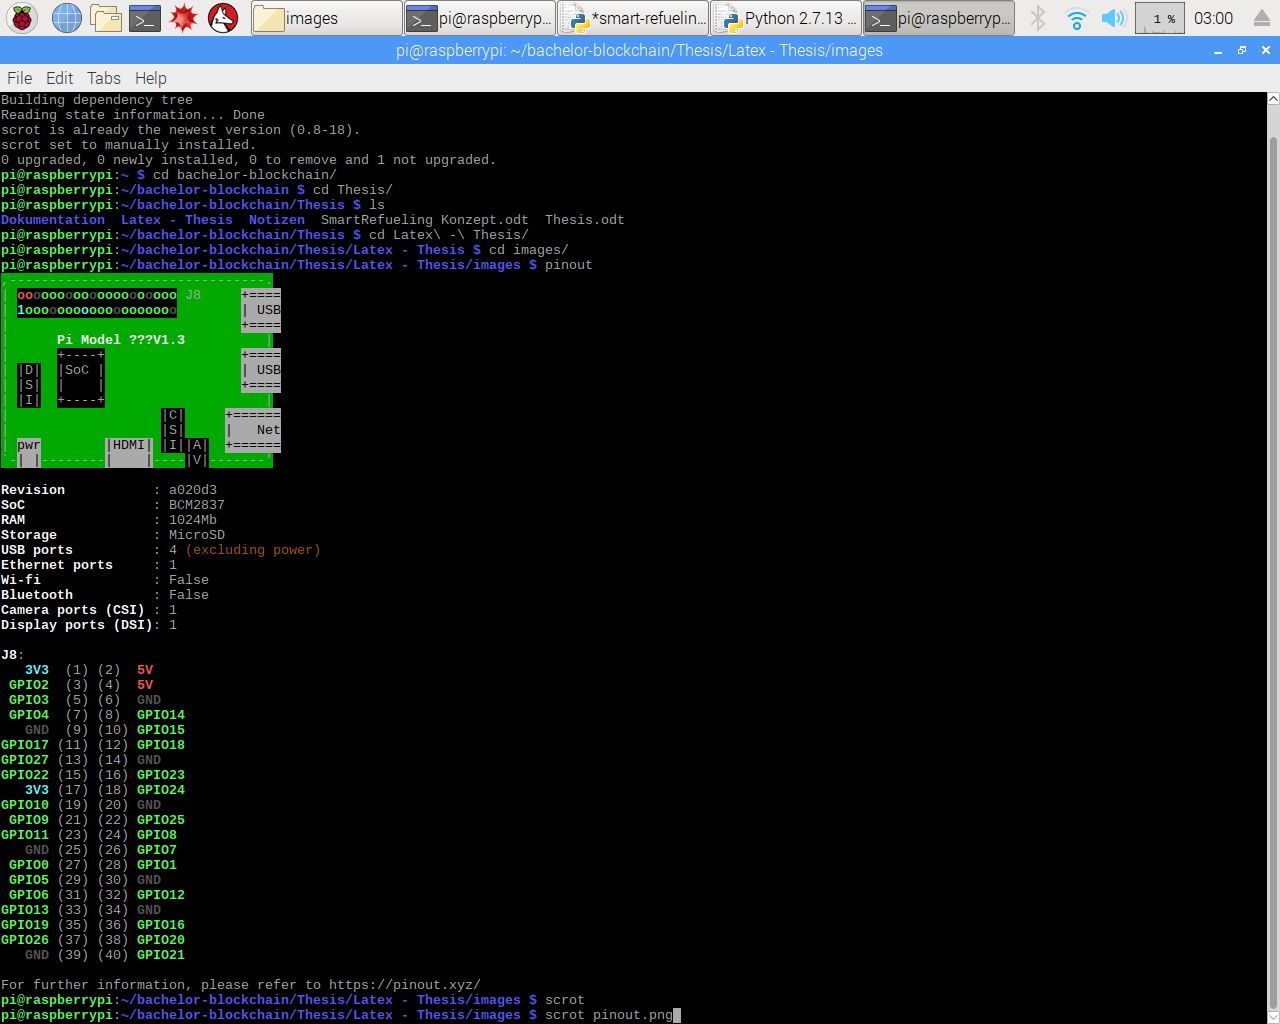
\includegraphics[scale=0.6]{pinout.png}%
\caption{Pinout-Ausgabe}
\end{figure}

Die Komponenten m�ssen in das Steckbrett gesteckt werden, sodass sie erreichbar bleiben, um sie zu verkabeln und zugleich nutzen zu k�nnen. F�r eine optimale �bersicht wurden die Komponenten mittig platziert.

F�r die Umsetzung m�ssen diese Komponenten f�r den Nutzer interagierbar sein, dazu werden sie mit zuf�lligen, freien GPIO-Pins verbunden.

\begin{table}[H]%
\centering
\begin{tabular}{l|l}
Komponente & GPIO-Pin\\
\hline
Button 1 & 11\\
Button 2 & 22\\
LED & 10
\end{tabular}
\caption{Korrespondenz der Buttons mit den GPIO-Pins}
\label{buttonlayout}
\end{table}

\subsubsection{PyOTA}
Bei PyOTA handelt es sich um eine Python-Bibliothek f�r IOTA. Sie implementiert die API und unterst�tzt Funktionalit�ten um eine Transaktion eigenst�ndig erstellen zu k�nnen\footnote{siehe dazu https://pyota.readthedocs.io/en/latest/}.

Um die Bibliothek f�r die Umsetzung zur Verf�gung zu stellen kann sie �ber das Paketverwaltungsprogramm f�r die Umgebung installiert werden.
\begin{lstlisting}[language=bash]
> pip install pyota
\end{lstlisting}

Eine wichtige Abh�ngigkeit (Dependancy) von PyOTA ist die Cryptography-Bibliothek. Diese wird nicht automatisch heruntergeladen und installiert, sondern dies muss manuell geschehen\footnote{mehr Informationen dazu https://cryptography.io/en/latest/installation/}.

Weiterhin muss angemerkt werden, das bei Raspbian kein System-Pfad zu den zus�tzlich installierten Paketen (per pip install) f�r Python2.7 gibt. Demzufolge muss der Pfad vor jedem Programmstart in das Suchverzeichnis hinzugef�gt werden. Dies geschieht mit folgendem Code:
\begin{lstlisting}[language=Python]
import sys
sys.path.append("/home/pi/.local/lib/python2.7/site-packages")  #path muss erweitert werden damit PyOta librarys gefunden werden k�nnen
\end{lstlisting}

\subsection{Ergebnis der Vorbereitung}
Nachdem alle Vorbedingungen erf�llt sind, ist der Raspberry Pi einsatzbereit um ein Programm zu erstellen und auszuf�hren, welches auf Benutzereingaben an Kn�pfen horcht, visuelles Feedback gibt und mit der PyOta-Bibliothek arbeitet.

\section{Umsetzung}
In diesem Abschnitt sollen die ausgew�hlten Programmierans�tze gezeigt und besprochen werden. Es soll ein �berblick �ber die verwendeten Methoden geschaffen werden. Bei mehreren m�glichen Methoden soll dar�ber hinaus deutlich werden, warum die entsprechende Methode gew�hlt wurde.

\subsection{GPIO-Pins}
Auf dem Raspberry Pi m�ssen die GPIO-Pins vorkonfiguriert werden um danach einzelne Pins als Inputs oder Outputs setzen zu k�nnen. Die Funktionalit�t wird der vorinstallierten RPi.GPIO-Bibliothek entnommen. Sie wird zur Abk�rzung fortan mit "`GPIO"' referenziert.
\begin{lstlisting}[language=Python]
import RPi.GPIO as GPIO     #importiere GPIO-Bibliothek f�r Ein-/Ausgaben von Inputs und Outputs (Buttons/LEDs)
\end{lstlisting}

Zum Ansprechen der Pins muss bestimmt werden, welche Pins mit welcher Nummer korrespondieren. Zum Beispiel hat Pin 12 eine Zweideutigkeit in dem Sinne, dass er zum einen Pin 12 bei einer, numerisch sortierten Aneinanderreihung, der zw�lfte Pin des Panels ist. Zum anderen kann sich Pin 12 auch auf den Namen des Pins beziehen, in diesem Beispiel "`GPIO12"', welcher sich nicht an einer numerischen Anordnung befindet.

Daher muss der Modus des Boards gesetzt werden mit folgender Code Zeile.
\begin{lstlisting}[language=Python]
GPIO.setmode(GPIO.BCM)
\end{lstlisting}
GPIO.BCM bezieht sich auf den Broadcom SOC (system on chip) Kanal, der angesprochen wird. Die Auswahl von dieser Variante hat keine Vor- oder Nachteile f�r das Projekt und wurde arbitr�r ausgew�hlt.

Nachdem der Modus eingestellt wurde kann nun die Datenrichtung der Pins bestimmt werden. Daf�r wird der Pin als Input oder als Output gesetzt.
\begin{lstlisting}[language=Python]
BUTTON1 = 11
BUTTON2 = 22
LED = 10

GPIO.setup(BUTTON1, GPIO.IN)
GPIO.setup(BUTTON2, GPIO.IN)
GPIO.setup(LED, GPIO.OUT, initial = False)
\end{lstlisting}

Nun sind die einzelnen Pins manipulierbar, bzw. auslesbar. Je nachdem ob man einen Output-Pin setzten m�chte oder einen Input-Pin auslesen m�chte, sind verschiedene Funktionen verwendbar.

Zum Auslesen ob ein Knopf gedr�ckt wurde bietet sich die folgende einfache Implementierung an. Das Programm wartet solange, bis der Knopf gedr�ckt und losgelassen wurde.
\begin{lstlisting}[language=Python]
def wait_for_button_click(button):
    while not GPIO.input(button):
        pass
    while GPIO.input(button):
        pass
\end{lstlisting}
Wobei der Parameter 'button' die Pin-Nummer referenziert.\\
Es bieten sich auch andere, effizientere Methoden an, jedoch ist diese Implementierung f�r den Prototypen ausreichend.

Um einen Output wie zum Beispiel die LED zu setzen, ben�tigen wir diese Code-Zeile:
\begin{lstlisting}[language=Python]
GPIO.output(LED, True)
\end{lstlisting}

\subsection{IOTA Einrichtung}
Unter der Einrichtung von IOTA ist zu verstehen, die IOTA-Bibliothek so zu utilisieren, dass mit der API eine Transaktion in das Tangle-Netzwerk ver�ffentlicht werden kann. F�r so eine Funktionalit�t bietet sich das Iota-Objekt an. Dieses wird dank des iota-Moduls bereitgestellt.
\begin{lstlisting}[language=Python]
from iota import Iota
\end{lstlisting}

Damit nun das Iota Objekt initialisiert werden kann, braucht es zwei Argumente. Den Seed, und eine Adresse zu einer Full-Node.

\paragraph{Seed} Der Seed "`DSPOAXMVSC99IUIVJXTIBZFATVFKTCLLJYOLAGSMFJGFXAWEB9GNTQWEDVRYHKIOQF9T9IZY9IVPKTSZK"' wurde aus einer zuf�lligen Kombination der Gro�buchstaben 'A-Z' und der Nummer 9 eigenh�ndig generiert und wird f�r den Prototypen genutzt. Im Programmcode ist der Seed hinterlegt, dies k�nnte bei einer realistischen Umgebung zu Sicherheitsrisiken f�hren, f�r die prototypische Umsetzung gen�gt es.

\paragraph{Full-Node} Aus einer Liste im Internet\footnote{siehe https://iotasalad.org/nodes}, in der einige Full-Nodes aufgelistet sind, wurde die folgende Adresse beliebig ausgesucht: https://potato.iotasalad.org:14265. Der Full-Node �bernimmt die Arbeit die erstellte Transaktion in das Tangle zu ver�ffentlichen, da der Raspberry Pi zu leistungsschwach ist um den Proof-Of-Work zeiteffizient zu �bernehmen.

Aus den gegebenen Parametern kann das Iota-Objekt erstellt werden.
\begin{lstlisting}[language=Python]
seed = "DSPOAXMVSC99IUIVJXTIBZFATVFKTCLLJYOLAGSMFJGFXAWEB9GNTQWEDVRYHKIOQF9T9IZY9IVPKTSZK"  
fullnode_url = "https://potato.iotasalad.org:14265"
api = Iota(fullnode_url, seed)
\end{lstlisting}

Es ist nun m�glich, grundlegende Funktionen wie Adressgenerierung nutzen zu k�nnen.

\subsection{IOTA Transaktion}
Um eine Transaktion zu erstellen werden f�r diese Implementierung die Klassen ProposedTransaction, ProposedBundle, Address, Tag und TryteString zus�tzlich zu Iota von dem iota-Modul genutzt.
\begin{lstlisting}[language=Python]
from iota import Iota, ProposedTransaction, ProposedBundle, Address, Tag, TryteString
\end{lstlisting}

Vorerst muss ein "`Vorabtransaktions"'-Objekt erstellt werden mit Adresse, Wert, Tag und Message.
\begin{lstlisting}[language=Python]
proposedTrx = ProposedTransaction(
    address = Address(reciever_address),
    value = 0,
    tag = Tag("BACHELORTEST"),
    message = TryteString.from_string("This is a test transaction")
)
proposedBundle = ProposedBundle([proposedTrx])
\end{lstlisting}
Das Transaktionsobjekt wird gef�llt mit der Empf�ngeradresse, dem Wert 0 (eine "`Meta Transaction"'), einem Tag welcher mithilfe des Tag-Objekts erstellt wird und einer beliebigen Nachricht, welche mithilfe von TryteString in Trits umgewandelt wird. Abschlie�end wird ein "`Vorabbundle"' erstellt, welches mit der Vorabtransaktion bef�llt wird.

Dieses Vorabbundle muss gepr�ft und signiert werden, daf�r wird es als Parameter an die vorher erstellte Iota-Instanz �bergeben. Der Aufruf gibt ein vorbereitetes Bundle zur�ck, welches mittels API-Aufruf an die Full-Node verschickt wird. Dort wird sie abschlie�end verarbeitet und in das Tangle-Netzwerk ver�ffentlicht.
\begin{lstlisting}[language=Python]
preparedBundle = api.prepare_transfer(proposedBundle)
publishedBundle = api.send_transfer(depth = 3, transfers = proposedBundle)
\end{lstlisting}

Die Hash des PublishedBundle-Objekts kann genutzt werden, um die Transaktion nachzuvollziehen\footnote{z.B auf https://iotasear.ch/}.

\subsection{Kommunikation mit Tankstelle}
Die Kommunikation mit der Tankstelle erfolgt �ber eine REST API. Dies ist vereinfacht betrachtet eine Schnittstelle auf die �ber HTTP zugegriffen werden kann. Hierf�r bietet sich das vorinstallierte requests-Modul an.
\begin{lstlisting}[language=Python]
import requests #importiere requests-Bibliothek um HTTP-Anfragen zu erstellen
\end{lstlisting}

Ein Beispiel eines Anwendungsfalles ist das Beenden des Tankvorgangs. Der Code hierf�r ist in einer Methode ausgelagert mit den Argumenten 'route' und 'carId'. Die 'route' ist die Schnittstelle die angesprochen werden soll, in diesem Beispiel "`endFueling"'. Die 'carId' ist eine von der Tankstelle zugewiesene Nummer. Das Beispiel verschickt eine Anfrage an den Server (die Tankstelle) mit einem Parameter, der Identifikationsnummer des Autos, und gibt die Antwort zur�ck.
\begin{lstlisting}[language=Python]
endFuelingData = call_api("endFueling", carId)

def call_api(route, carId):
		params = {
				"id": carId
		}
	response = requests.get(fueling_url + route, params)
return response.json()
\end{lstlisting}

\chapter{Fahrzeug - Client}
Das Programm soll f�r einen realit�tsnahen Anwendungsfall auf einem relativ leistungsschwachen System arbeiten k�nnen. Daher liegt es nahe f�r die Programmierung des Programmierteils, der f�r das Tanken und Bezahlen mit IOTAs zust�ndig ist, einen Raspberry Pi anzusteuern.

Der Raspberry Pi soll in dieser prototypischen Umsetzung die Steuereinheit eines zuk�nftigen Autos ersetzen. Es soll mittels zwei Kn�pfen bedienbar sein, die die Steuerelemente in der Armatur des Autos darstellen sollen.

Da der Anspruch an starke Rechenleistung in einem Auto nicht zu hoch sein sollte (um zum Beispiel Kosten zu minimieren) ist es sinnvoll, keinen IOTA Full-Node zu betrieben, sondern nur einen Light-Node, der die Arbeit an einen Full-Node delegiert. Die Limitation der Hardware-Ressourcen ist ein Grund f�r die Umsetzung auf einem Raspberry Pi.

Die Anforderungen an das Smartauto sind wie folgt:
\begin{itemize}
	\item Der Nutzer muss vor dem dem Tankvorgang �ber die Tankstelle informiert werden
	\item Der Nutzer soll mit einem Knopfdruck tanken k�nnen
	\item Der Nutzer soll mit einem Knopfdruck bezahlen k�nnen, ohne das weitere Eingaben notwendig sind
	\item Die Transaktion muss schnell von der Tankstelle validiert werden
\end{itemize}
An diese Anforderungen orientiert sich die folgende Umsetzung.


\section{Aufbau}
Unter diesem Aspekt wird der Aufbau und die Einrichtung der einzelnen Komponenten beschrieben die f�r die Umsetzung n�tig sind.

\subsection{Vorbedingungen}
Unter diesem Aspekt werden die Voraussetzungen f�r die Umsetzung der clientseitigen Tankanwendung beschrieben. Diese Vorbedingungen wurden genutzt um den Raspberry Pi so einzurichten und zu konfigurieren, damit das Ger�t die Anforderungen an das Programm erf�llen kann.

Um die prototypische Anwendung umsetzen zu k�nnen, werden folgende Komponenten genutzt:

\subsubsection{Raspberry Pi 3 Model B}
Auf dem Raspberry Pi wird die Anwendung ausgef�hrt, Daten des Benutzers verarbeitet und Anfragen auf Webservices vollzogen. Auch die Transaktionen von IOTAs sollen mithilfe des CPUs erstellt werden.

\subsubsection{Steckbrett}
Das Steckbrett dient der Verbindung von Bedienelementen mit den GPIO-Pins des Raspberry Pis. Die Kn�pfe f�r die Bedienung der Tank-Anwendung werden auf diesem befestigt und mit den GPIO-Pins elektronisch verbunden.

\subsubsection{Micro SD Karte}
Diese Speicherkarte wird f�r den Raspberry Pi gebraucht. Auf dieser befindet sich das Betriebssystem mit dem der Raspberry Pi erst genutzt werden kann. Auch das Programm und sonstige Benutzerdaten werden auf dieser Speicherkarte gespeichert.

\subsubsection{Micro USB Netzteil 5,1 Volt 3,1 Ampere}
Der Raspberry Pi muss mittels eines Micro USB Eingangs mit Strom versorgt werden. Das Netzteil sollte eine Ausgangsspannung von mindestens 5,1 Volt aufweisen und es werden mindestens 2,5 Ampere empfohlen\footnote{Nach https://www.raspberrypi.org/documentation/hardware/raspberrypi/power/README.md}.

\subsubsection{5x Weiblich-M�nnlich Kabel, 2x M�nnlich-M�nnlich Kabel}
Verbindungskabel f�r das Steckbrett um elektronische Komponenten miteinander zu Verbinden.

\subsubsection{2x Taster, 1x Rote LED}
Elektronische Komponenten um dem Benutzer der Anwendung Bedienelemente zur Verf�gung zu stellen. Die LED dient f�r ein visuelles Feedback.

\subsubsection{Widerst�nde 1x 330 Ohm, 2x 10.000 Ohm, 2x 1.000 Ohm}
Die Widerst�nde sind f�r den kontrollierten Stromfluss unentbehrlich und sie verhindern, dass die Komponenten durch zu hohen Stromfluss besch�digt werden.

\subsection{Einrichtung}
Um den Raspberry Pi so einzurichten, dass es m�glich ist, Anwendungen zu programmieren und zu testen, sollte dieser mittels eines HDMI-Kabels an einen Monitor angeschlossen werden. Weiterhin sollten Peripherieger�te wie Tastatur und Maus �ber die USB-Ausg�nge angeschlossen werden um sich durch die Bedienoberfl�che navigieren zu k�nnen. Doch damit das Ger�t vollst�ndig bedienbar wird, muss es mit einem Betriebssystem ausgestattet sein. Aufgrund von offiziellem Support seitens der Raspberry Pi Foundation [26](Quelle) wurde das Raspbian Betriebssystem f�r die Umsetzung ausgew�hlt. Bei Raspbian handelt es sich um ein, auf Linux basierendes Betriebssystem, welches von der Raspberry Pi Foundation ver�ffentlicht wurde.

Das Raspbian Betriebssystem muss auf die Micro SD Karte geladen werden, damit es f�r den Raspberry Pi zur Verf�gung steht. In folgenden Schritten wurde die Speicherkarte mit Raspbian beschrieben:
\begin{enumerate}
	\item Download von Raspbian (https://www.raspberrypi.org/downloads/)
	\item Gegebenenfalls .zip/.rar entpacken
	\item Speicherkarte in ein Kartenleseger�t stecken
	\item Mithilfe eines Brennprogramms die Imagedatei auf die Speicherkarte brennen (flashen)
\end{enumerate}

Die Speicherkarte ist nun formatiert und mit Raspbian ausgestattet, sie kann nun aus dem Kartenleseger�t genommen werden und in den Raspberry Pi gesteckt werden.

Nachdem das Ger�t zum ersten Mal gestartet wird, muss das Betriebssystem einmalig eingerichtet werden. Wenn dies geschehen ist, sollte man jegliche Software-Pakete in Raspbian updaten um m�gliche Fehler vorzubeugen. Dies kann mit folgenden Befehlen in dem Terminal des Betriebssystems vollzogen werden:

\begin{lstlisting}[language=bash]
> sudo apt-get update
> sudo apt-get dist-upgrade
\end{lstlisting}

\subsubsection{Steckbrett und GPIO-Pins}
Die Taster und LEDs m�ssen elektrisch mit den GPIO-Pins verbunden werden, um von dem Raspberry Pi angesprochen werden zu k�nnen. Die Taster stellen Kn�pfe auf der Armatur des Autos dar. Die LED dient daf�r, ein visuelles Feedback zu geben, zum Beispiel im Bezug auf die Tank-Anwendung ob nun getankt werden kann.

Daf�r ist es n�tzlich, mit dem Pin-Layout des Raspberry Pis vertraut zu sein. Mit dem Terminal-Befehl

\begin{lstlisting}[language=bash]
> pinout
\end{lstlisting}

ist es m�glich einen �berblick �ber das Layout des Raspberry Pis zu erhalten. Auch die Benennung der einzelnen Pins ist aufgef�hrt.

\begin{figure}[H]%
\centering
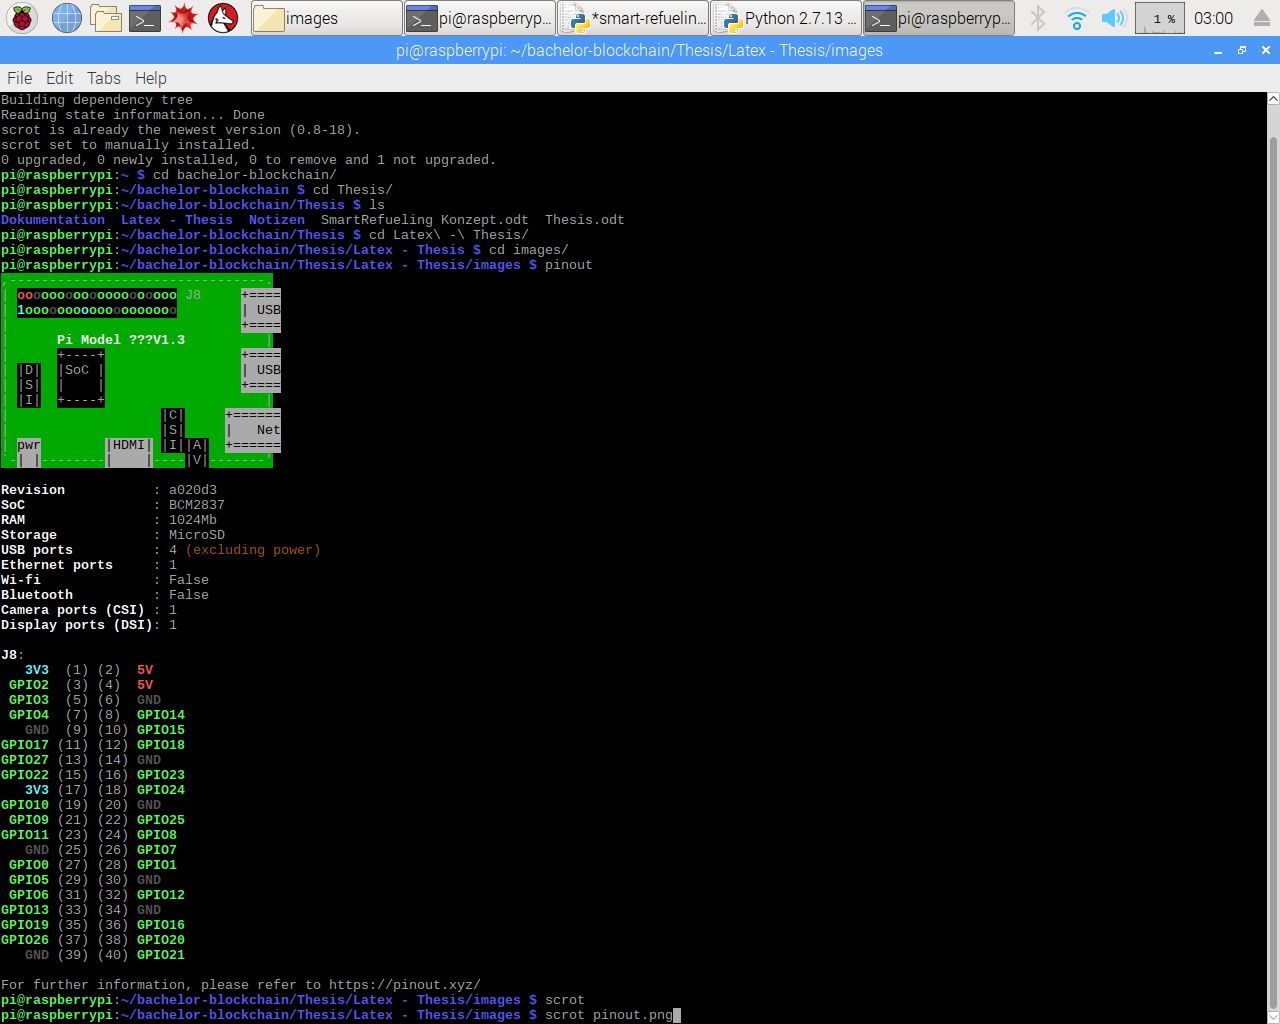
\includegraphics[scale=0.6]{pinout.png}%
\caption{Pinout-Ausgabe}
\end{figure}

Die Komponenten m�ssen in das Steckbrett gesteckt werden, sodass sie erreichbar bleiben, um sie zu verkabeln und zugleich nutzen zu k�nnen. F�r eine optimale �bersicht wurden die Komponenten mittig platziert.

F�r die Umsetzung m�ssen diese Komponenten f�r den Nutzer interagierbar sein, dazu werden sie mit zuf�lligen, freien GPIO-Pins verbunden.

\begin{table}[H]%
\centering
\begin{tabular}{l|l}
Komponente & GPIO-Pin\\
\hline
Button 1 & 11\\
Button 2 & 22\\
LED & 10
\end{tabular}
\caption{Korrespondenz der Buttons mit den GPIO-Pins}
\label{buttonlayout}
\end{table}

\subsubsection{PyOTA}
Bei PyOTA handelt es sich um eine Python-Bibliothek f�r IOTA. Sie implementiert die API und unterst�tzt Funktionalit�ten um eine Transaktion eigenst�ndig erstellen zu k�nnen\footnote{siehe dazu https://pyota.readthedocs.io/en/latest/}.

Um die Bibliothek f�r die Umsetzung zur Verf�gung zu stellen kann sie �ber das Paketverwaltungsprogramm f�r die Umgebung installiert werden.
\begin{lstlisting}[language=bash]
> pip install pyota
\end{lstlisting}

Eine wichtige Abh�ngigkeit (Dependancy) von PyOTA ist die Cryptography-Bibliothek. Diese wird nicht automatisch heruntergeladen und installiert, sondern dies muss manuell geschehen\footnote{mehr Informationen dazu https://cryptography.io/en/latest/installation/}.

Weiterhin muss angemerkt werden, das bei Raspbian kein System-Pfad zu den zus�tzlich installierten Paketen (per pip install) f�r Python2.7 gibt. Demzufolge muss der Pfad vor jedem Programmstart in das Suchverzeichnis hinzugef�gt werden. Dies geschieht mit folgendem Code:
\begin{lstlisting}[language=Python]
import sys
sys.path.append("/home/pi/.local/lib/python2.7/site-packages")  #path muss erweitert werden damit PyOta librarys gefunden werden k�nnen
\end{lstlisting}

\subsection{Ergebnis der Vorbereitung}
Nachdem alle Vorbedingungen erf�llt sind, ist der Raspberry Pi einsatzbereit um ein Programm zu erstellen und auszuf�hren, welches auf Benutzereingaben an Kn�pfen horcht, visuelles Feedback gibt und mit der PyOta-Bibliothek arbeitet.

\section{Umsetzung}
In diesem Abschnitt sollen die ausgew�hlten Programmierans�tze gezeigt und besprochen werden. Es soll ein �berblick �ber die verwendeten Methoden geschaffen werden. Bei mehreren m�glichen Methoden soll dar�ber hinaus deutlich werden, warum die entsprechende Methode gew�hlt wurde.

\subsection{GPIO-Pins}
Auf dem Raspberry Pi m�ssen die GPIO-Pins vorkonfiguriert werden um danach einzelne Pins als Inputs oder Outputs setzen zu k�nnen. Die Funktionalit�t wird der vorinstallierten RPi.GPIO-Bibliothek entnommen. Sie wird zur Abk�rzung fortan mit "`GPIO"' referenziert.
\begin{lstlisting}[language=Python]
import RPi.GPIO as GPIO     #importiere GPIO-Bibliothek f�r Ein-/Ausgaben von Inputs und Outputs (Buttons/LEDs)
\end{lstlisting}

Zum Ansprechen der Pins muss bestimmt werden, welche Pins mit welcher Nummer korrespondieren. Zum Beispiel hat Pin 12 eine Zweideutigkeit in dem Sinne, dass er zum einen Pin 12 bei einer, numerisch sortierten Aneinanderreihung, der zw�lfte Pin des Panels ist. Zum anderen kann sich Pin 12 auch auf den Namen des Pins beziehen, in diesem Beispiel "`GPIO12"', welcher sich nicht an einer numerischen Anordnung befindet.

Daher muss der Modus des Boards gesetzt werden mit folgender Code Zeile.
\begin{lstlisting}[language=Python]
GPIO.setmode(GPIO.BCM)
\end{lstlisting}
GPIO.BCM bezieht sich auf den Broadcom SOC (system on chip) Kanal, der angesprochen wird. Die Auswahl von dieser Variante hat keine Vor- oder Nachteile f�r das Projekt und wurde arbitr�r ausgew�hlt.

Nachdem der Modus eingestellt wurde kann nun die Datenrichtung der Pins bestimmt werden. Daf�r wird der Pin als Input oder als Output gesetzt.
\begin{lstlisting}[language=Python]
BUTTON1 = 11
BUTTON2 = 22
LED = 10

GPIO.setup(BUTTON1, GPIO.IN)
GPIO.setup(BUTTON2, GPIO.IN)
GPIO.setup(LED, GPIO.OUT, initial = False)
\end{lstlisting}

Nun sind die einzelnen Pins manipulierbar, bzw. auslesbar. Je nachdem ob man einen Output-Pin setzten m�chte oder einen Input-Pin auslesen m�chte, sind verschiedene Funktionen verwendbar.

Zum Auslesen ob ein Knopf gedr�ckt wurde bietet sich die folgende einfache Implementierung an. Das Programm wartet solange, bis der Knopf gedr�ckt und losgelassen wurde.
\begin{lstlisting}[language=Python]
def wait_for_button_click(button):
    while not GPIO.input(button):
        pass
    while GPIO.input(button):
        pass
\end{lstlisting}
Wobei der Parameter 'button' die Pin-Nummer referenziert.\\
Es bieten sich auch andere, effizientere Methoden an, jedoch ist diese Implementierung f�r den Prototypen ausreichend.

Um einen Output wie zum Beispiel die LED zu setzen, ben�tigen wir diese Code-Zeile:
\begin{lstlisting}[language=Python]
GPIO.output(LED, True)
\end{lstlisting}

\subsection{IOTA Einrichtung}
Unter der Einrichtung von IOTA ist zu verstehen, die IOTA-Bibliothek so zu utilisieren, dass mit der API eine Transaktion in das Tangle-Netzwerk ver�ffentlicht werden kann. F�r so eine Funktionalit�t bietet sich das Iota-Objekt an. Dieses wird dank des iota-Moduls bereitgestellt.
\begin{lstlisting}[language=Python]
from iota import Iota
\end{lstlisting}

Damit nun das Iota Objekt initialisiert werden kann, braucht es zwei Argumente. Den Seed, und eine Adresse zu einer Full-Node.

\paragraph{Seed} Der Seed "`DSPOAXMVSC99IUIVJXTIBZFATVFKTCLLJYOLAGSMFJGFXAWEB9GNTQWEDVRYHKIOQF9T9IZY9IVPKTSZK"' wurde aus einer zuf�lligen Kombination der Gro�buchstaben 'A-Z' und der Nummer 9 eigenh�ndig generiert und wird f�r den Prototypen genutzt. Im Programmcode ist der Seed hinterlegt, dies k�nnte bei einer realistischen Umgebung zu Sicherheitsrisiken f�hren, f�r die prototypische Umsetzung gen�gt es.

\paragraph{Full-Node} Aus einer Liste im Internet\footnote{siehe https://iotasalad.org/nodes}, in der einige Full-Nodes aufgelistet sind, wurde die folgende Adresse beliebig ausgesucht: https://potato.iotasalad.org:14265. Der Full-Node �bernimmt die Arbeit die erstellte Transaktion in das Tangle zu ver�ffentlichen, da der Raspberry Pi zu leistungsschwach ist um den Proof-Of-Work zeiteffizient zu �bernehmen.

Aus den gegebenen Parametern kann das Iota-Objekt erstellt werden.
\begin{lstlisting}[language=Python]
seed = "DSPOAXMVSC99IUIVJXTIBZFATVFKTCLLJYOLAGSMFJGFXAWEB9GNTQWEDVRYHKIOQF9T9IZY9IVPKTSZK"  
fullnode_url = "https://potato.iotasalad.org:14265"
api = Iota(fullnode_url, seed)
\end{lstlisting}

Es ist nun m�glich, grundlegende Funktionen wie Adressgenerierung nutzen zu k�nnen.

\subsection{IOTA Transaktion}
Um eine Transaktion zu erstellen werden f�r diese Implementierung die Klassen ProposedTransaction, ProposedBundle, Address, Tag und TryteString zus�tzlich zu Iota von dem iota-Modul genutzt.
\begin{lstlisting}[language=Python]
from iota import Iota, ProposedTransaction, ProposedBundle, Address, Tag, TryteString
\end{lstlisting}

Vorerst muss ein "`Vorabtransaktions"'-Objekt erstellt werden mit Adresse, Wert, Tag und Message.
\begin{lstlisting}[language=Python]
proposedTrx = ProposedTransaction(
    address = Address(reciever_address),
    value = 0,
    tag = Tag("BACHELORTEST"),
    message = TryteString.from_string("This is a test transaction")
)
proposedBundle = ProposedBundle([proposedTrx])
\end{lstlisting}
Das Transaktionsobjekt wird gef�llt mit der Empf�ngeradresse, dem Wert 0 (eine "`Meta Transaction"'), einem Tag welcher mithilfe des Tag-Objekts erstellt wird und einer beliebigen Nachricht, welche mithilfe von TryteString in Trits umgewandelt wird. Abschlie�end wird ein "`Vorabbundle"' erstellt, welches mit der Vorabtransaktion bef�llt wird.

Dieses Vorabbundle muss gepr�ft und signiert werden, daf�r wird es als Parameter an die vorher erstellte Iota-Instanz �bergeben. Der Aufruf gibt ein vorbereitetes Bundle zur�ck, welches mittels API-Aufruf an die Full-Node verschickt wird. Dort wird sie abschlie�end verarbeitet und in das Tangle-Netzwerk ver�ffentlicht.
\begin{lstlisting}[language=Python]
preparedBundle = api.prepare_transfer(proposedBundle)
publishedBundle = api.send_transfer(depth = 3, transfers = proposedBundle)
\end{lstlisting}

Die Hash des PublishedBundle-Objekts kann genutzt werden, um die Transaktion nachzuvollziehen\footnote{z.B auf https://iotasear.ch/}.

\subsection{Kommunikation mit Tankstelle}
Die Kommunikation mit der Tankstelle erfolgt �ber eine REST API. Dies ist vereinfacht betrachtet eine Schnittstelle auf die �ber HTTP zugegriffen werden kann. Hierf�r bietet sich das vorinstallierte requests-Modul an.
\begin{lstlisting}[language=Python]
import requests #importiere requests-Bibliothek um HTTP-Anfragen zu erstellen
\end{lstlisting}

Ein Beispiel eines Anwendungsfalles ist das Beenden des Tankvorgangs. Der Code hierf�r ist in einer Methode ausgelagert mit den Argumenten 'route' und 'carId'. Die 'route' ist die Schnittstelle die angesprochen werden soll, in diesem Beispiel "`endFueling"'. Die 'carId' ist eine von der Tankstelle zugewiesene Nummer. Das Beispiel verschickt eine Anfrage an den Server (die Tankstelle) mit einem Parameter, der Identifikationsnummer des Autos, und gibt die Antwort zur�ck.
\begin{lstlisting}[language=Python]
endFuelingData = call_api("endFueling", carId)

def call_api(route, carId):
		params = {
				"id": carId
		}
	response = requests.get(fueling_url + route, params)
return response.json()
\end{lstlisting}


\chapter{Ergebnis der Umsetzung}
Was aus den vorherigen Abschnitten folgt, ist ein Programm, welches mit einem Server �ber eine Rest-Schnittstelle kommuniziert und eigenst�ndig eine Transaktion ausf�hren kann. Mit dieser Applikation werden die Bezahlvorg�nge mit IOTAs abgewickelt. Um das Ergebnis zu veranschaulichen wird das Programm ausgef�hrt.

Die API wird im ersten Schritt gestartet. Sollte die Verbindung zu der Datenbank gelingen erscheint die Nachricht, dass die API gestartet sei und auf den Port 1717 h�rt.
\begin{figure}[H]%
\centering
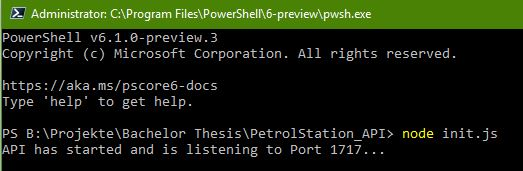
\includegraphics[scale=0.90]{startAPI.JPG}%
\caption{Zu sehen ist der Start des Servers}%
\label{fig:startapi}%
\end{figure}

Nun ist die Tankstelle einsatzbereit und wartet auf ihren ersten Kunden. Der Client auf dem Raspberry Pi wird ausgef�hrt und stellt mit dem Start des Programms einen Kunden dar, der an eine Zapfs�ule gefahren ist und nun tanken m�chte. Das Programm f�hrt vorerst einen Balance-Check durch. Die Anzahl der zugeh�rigen IOTAs wird ermittelt. Daraufhin fordert der Client Informationen zu der Tankstelle und des gew�nschten Kraftstoffes an. Das simulierte Auto ist ein Elektrofahrzeug.

Der Server antwortet mit einem JSON-Objekt.
\begin{lstlisting}
{
    "Super": {
        "cost": "22",
        "unit": "liter"
    },
    "SuperE10": {
        "cost": "15",
        "unit": "liter"
    },
    "Diesel": {
        "cost": "10",
        "unit": "liter"
    },
    "ENERGY-SB": {
        "cost": "2",
        "unit": "kwH"
    }
}
\end{lstlisting}
("`ENERGY-SB"' ist in diesem Falle ein fiktiver Markenname des Stroms.)

Daraufhin, simuliert der Nutzer des Prototypen mit einem Knopfdruck, dass er den passenden Zapfhahn in das Auto eingef�hrt hat. Das Programm erkennt an welcher Zapfs�ulennummer und an welchem Kraftstoff das Auto angesteckt ist und gibt diese an den Server weiter. Damit kann der Server wissen, welche Zapfs�ule zu dem Auto geh�rt und weist dem Auto eine Identifikationsnummer zu. Dies ist erforderlich, damit die Tankstelle dem richtigen Auto die entsprechende Rechnung ausstellen kann. Die Antwort der Tankstelle sieht wie folgt aus:
\begin{lstlisting}
{
	"id": 1539567699
}
\end{lstlisting}

Mit dem Erhalt der ID kann das Fahrzeug nun getankt werden. Dies wird visuell durch eine aufblinkende LED zus�tzlich verdeutlicht.

\begin{figure}[H]%
\centering
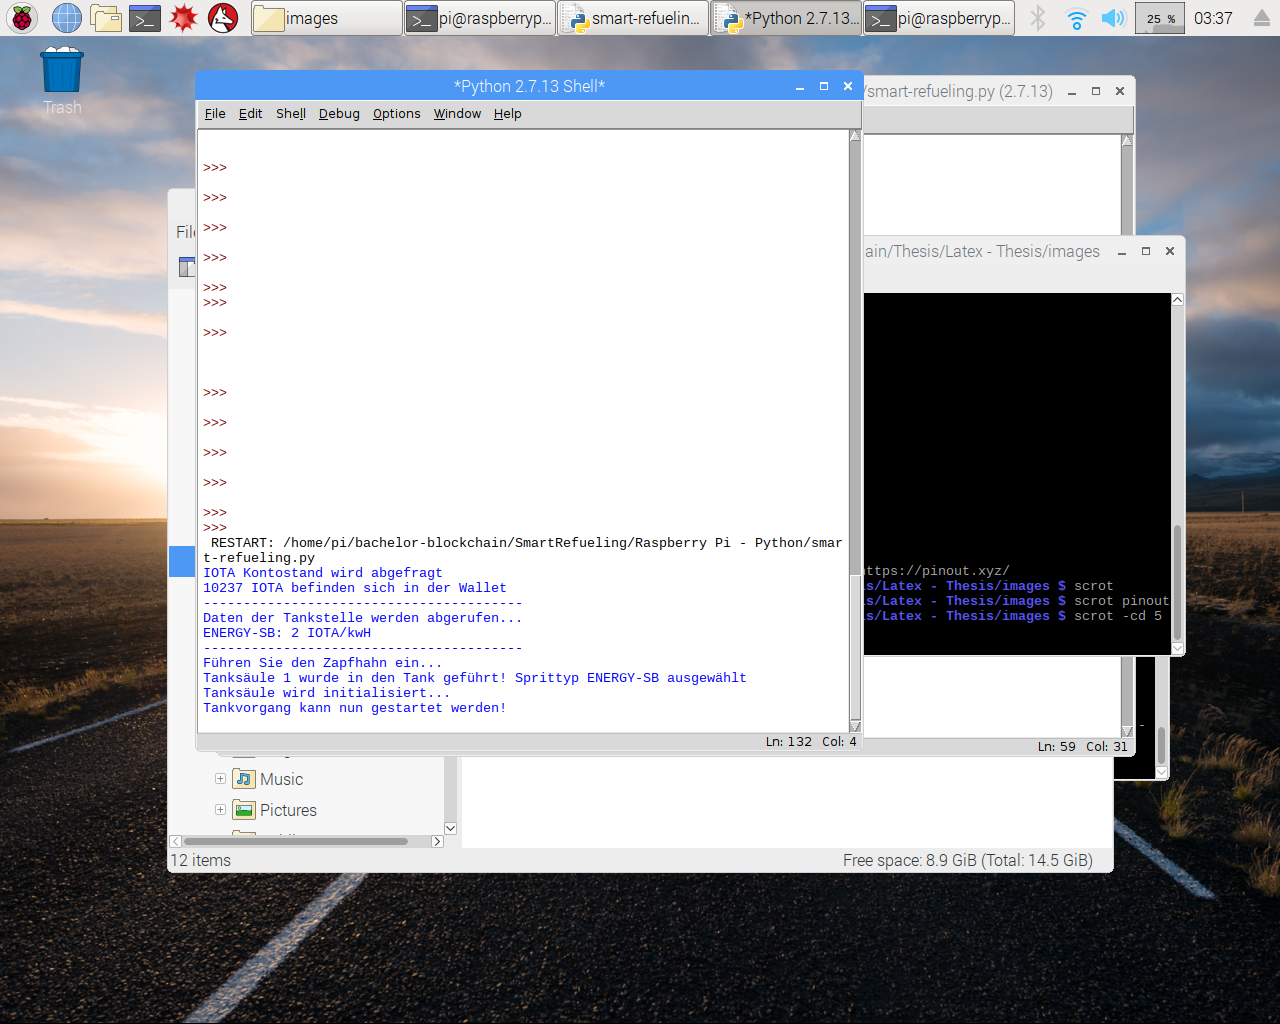
\includegraphics[scale=1.0]{tankbereit.png}%
\caption{Ausgabe in der Konsole wenn das Auto tankbereit ist}
\end{figure}

\begin{figure}[H]%
\centering
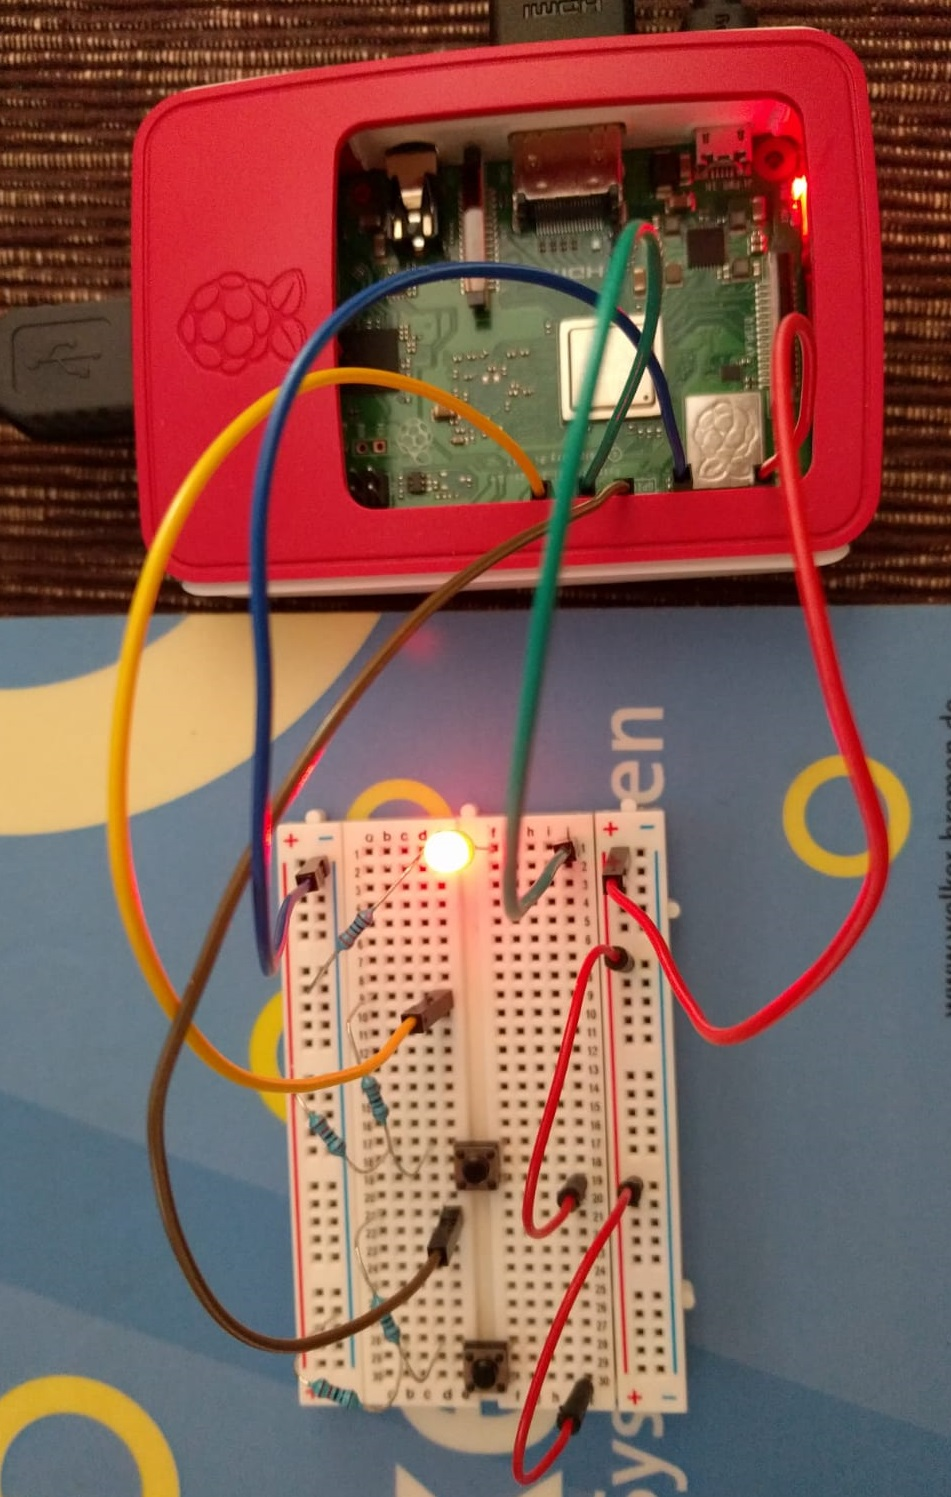
\includegraphics[scale=0.4]{reallife.jpg}%
\caption{Zu sehen ist das Steckbrett der Anwendung, die LED-Leuchtet}
\end{figure}

Wenn nun der Button 1 gedr�ckt wird, wird das Auto solange getankt bis der Nutzer entweder losgelassen hat, oder nicht mehr gen�gend IOTAs zur Verf�gung stehen. Das tanken wird mit einer Anfrage zum Server gestartet. Diese Art der Implementierung wurde ausgew�hlt, da die Prototyp-Tankstelle anders keine Informationen �ber den Tankvorgang erhalten w�rde ohne einen hohen Aufwand mit dem Abbilden einer Tanks�ule zu erzielen. Es ist anzumerken, dass diese Implementierung nur f�r eine prototypische Umsetzung ist und der Fokus auf die Bezahlung mit IOTAs liegt.

Mit der Anfrage den Tankvorgang zu starten, z�hlt die Tankstelle einen Z�hler solange hoch bis eine pauseFueling-Anfrage gestellt wird. Der Z�hler stellt die getankte Menge des Kraftstoffes dar. Mit einer getFueling-Anfrage kann diese Menge periodisch abgefragt werden.

\begin{figure}[H]%
\centering
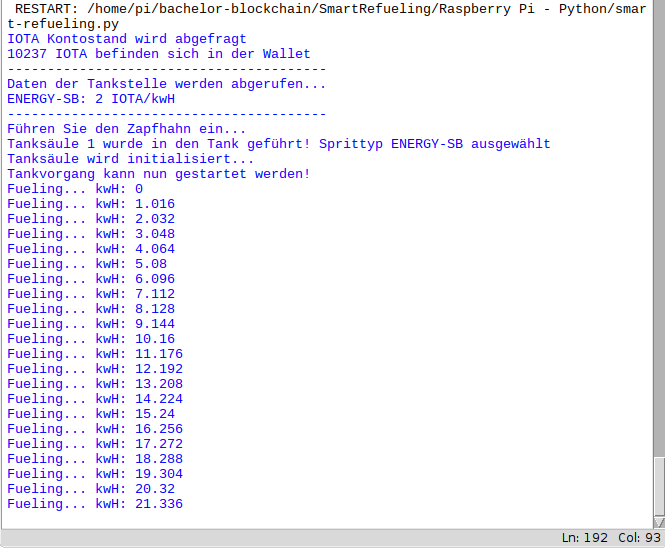
\includegraphics[scale=0.8]{tankvorgang.png}%
\caption{Dargestellt ist wie der Server periodisch die Tankf�llung wiedergibt}
\end{figure}

Mit einem Knopfdruck auf Button 2 wird der Tankvorgang mit einer endFueling-Anfrage beendet und der Nutzer bekommt unter anderem die Empf�nger-Adresse gestellt. Die Bezahlung wird im Hintergrund abgewickelt und der Nutzer kann weiterfahren.
\begin{lstlisting}
{
	"data": {
		"fuel_type": "ENERGY-SB",
        	"cost": 44.704,
        	"amount": 22.352,
        	"initTimestamp": 1539567699812,
        	"id": 1539567699,
        	"start_fueling_at": 1539568031583,
        	"end_fueling_at": 1539568172019,
        	"unit": "kwH",
        	"address": "LOZMZOKJWWVASYYWT999JPLDBMUSFZKMLZW9IXHTOAUOQKZMRLRAZCWECAFONWKT9HSHKHLMKAWSQFFXX"
    	}
}
\end{lstlisting}

\begin{figure}[H]%
\centering
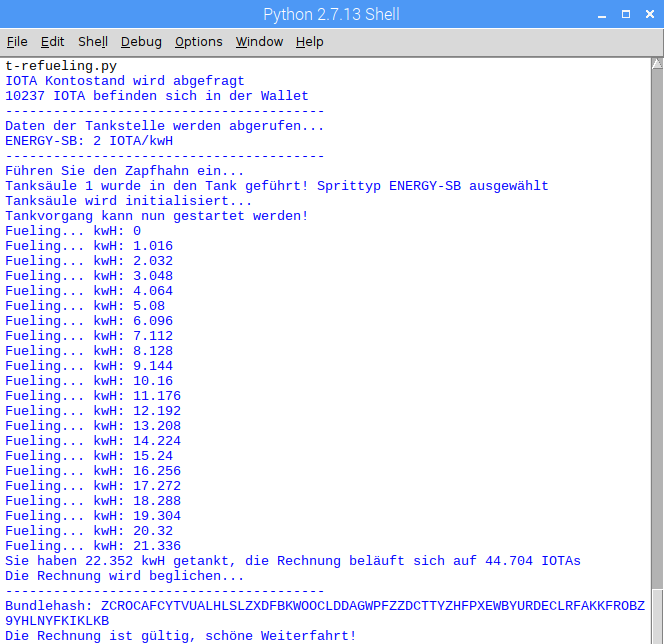
\includegraphics[scale=0.8]{bezahlen.png}%
\caption{Das Ende der Transaktion wird gezeigt}
\end{figure}

Zur �berpr�fung wird der Bundle-Hash ausgegeben. Dieser kann auf der Internetseite www.thetangle.org eingeben und nachvollziehen werden. Bei nicht Best�tigung kann das Bundle direkt auf der Webseite re-attached werden.

\begin{figure}[H]%
\centering
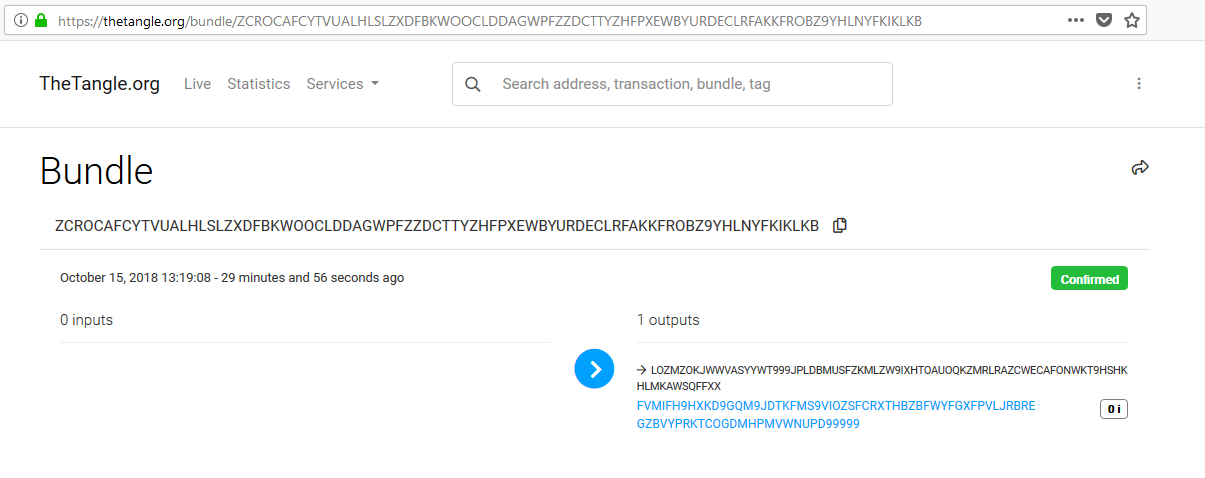
\includegraphics[scale=0.4]{bundle.PNG}%
\caption{Das Bundle ist auf der Webseite einsehbar}
\end{figure}

\begin{figure}[H]%
\centering
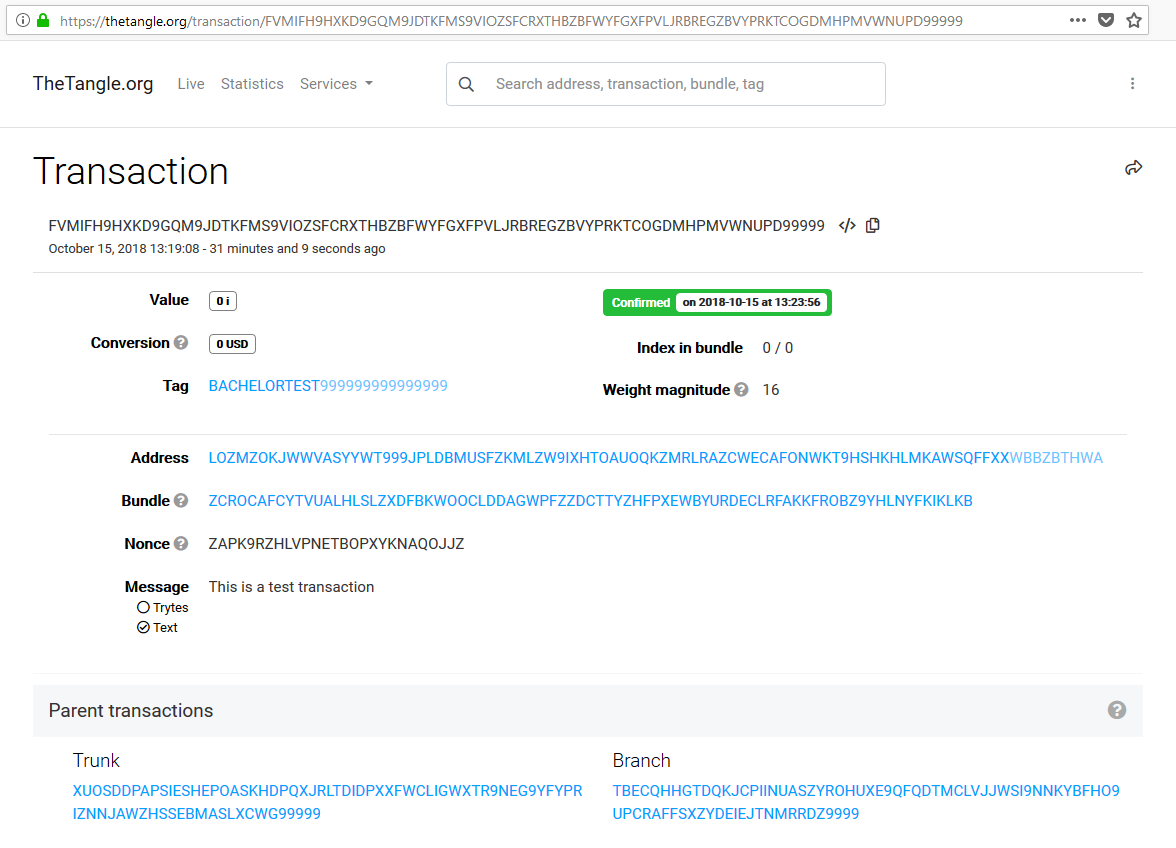
\includegraphics[scale=0.4]{trx.PNG}%
\caption{Auch die Transaktion ist auf der Webseite nachzuvollziehen}
\end{figure}

Die prototypische Umsetzung ist damit erfolgreich beendet. Es wurde gezeigt wie eine Implementierung einer Distributed Ledger Technologie (DLT) aussehen k�nnte. Das Programm verwendet IOTA um Zahlungen zu erstellen, wegen dem Wegfall der Transaktionsgeb�hren. Damit ist ein Beispiel einer zuk�nftigen Nutzung einer DLT gegeben, welches die zugrundeliegende Fragestellung in der Hinsicht unterst�tzt, dass im Aspekt der N�tzlichkeit und Programmierbarkeit eine Zukunftstauglichkeit vorliegt.


